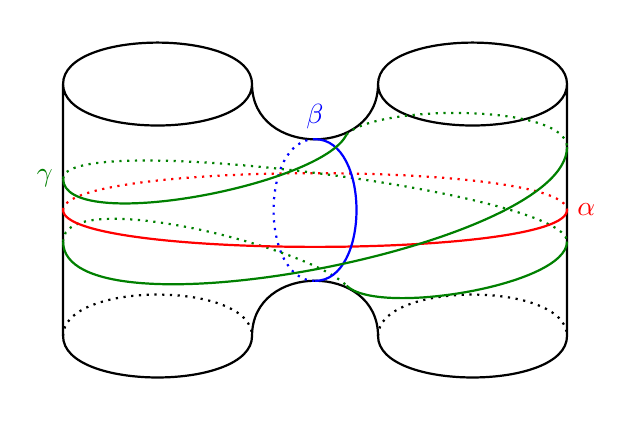
\begin{tikzpicture}[scale=0.4, thick]
    \coordinate (NWL) at (-20, 13);
    \coordinate (NWR) at (-14, 13);
    \coordinate (NEL) at (-10, 13);
    \coordinate (NER) at (-4, 13);
    \coordinate (SWL) at (-20, 5);
    \coordinate (SWR) at (-14, 5);
    \coordinate (SEL) at (-10, 5);
    \coordinate (SER) at (-4, 5);
    \coordinate (N) at (-12, 11.25);
    \coordinate (S) at (-12, 6.75);
    \coordinate (W) at (-20, 9);
    \coordinate (E) at (-4, 9);
    
    \draw (NWL) to [out=90, in=90, looseness=0.75] (NWR);
    \draw (NEL) to [out=90, in=90, looseness=0.75] (NER);
    
    \draw (NWL) 
        to [out=270, in=270, looseness=0.75] (NWR)
        to [out=270, in=270, looseness=1.50] (NEL)
        to [out=270, in=270, looseness=0.75] (NER)
        to (SER)
        to [out=270, in=270, looseness=0.75] (SEL)
        to [out=90, in=90, looseness=1.50] (SWR)
        to [out=270, in=270, looseness=0.75] (SWL)
        to (NWL);

    \draw [dotted, in=90, out=90, looseness=0.75] (SEL) to (SER);
    \draw [dotted, in=90, out=90, looseness=0.75] (SWL) to (SWR);
    
    \draw [red, dotted, bend left=90, looseness=0.25] (W) to (E);
    \draw [blue, dotted, bend right=90] (N) to (S);
    \draw [Green, dotted] (-20, 10) [out=90, in=90, looseness=0.25] to (-4, 8);
    \draw [Green, dotted] (-11, 11.4) [out=45, in=90, looseness=0.5] to (-4, 11);
    \draw [Green, dotted] (-20, 8) [out=90, in=135, looseness=0.5] to (-11, 6.6);


    \draw [red, bend right=90, looseness=0.25] (W) to (E) node [right] {$\alpha$};
    \draw [blue, bend left=90] (N) node [above] {$\beta$} to (S);
    \draw [Green] (-11, 11.4) [out=245, in=270, looseness=0.5] to (-20, 10) node [left] {$\gamma$};
    \draw [Green] (-4, 11) [out=270, in=270, looseness=0.5] to (-20, 8);
    \draw [Green] (-11, 6.6) [out=-45, in=270, looseness=0.5] to (-4, 8);

\end{tikzpicture}